
%(BEGIN_QUESTION)
% Copyright 2006, Tony R. Kuphaldt, released under the Creative Commons Attribution License (v 1.0)
% This means you may do almost anything with this work of mine, so long as you give me proper credit

Reguleringsventiler brukt i pneumatiske og hydrauliske fluidkraftsystemer har ofte en {\it spool}-mekanisme (spole), og skjemasymbolene for slike spoolventiler er ganske ulike ventilsymbolene i P\&ID-er og sløyfediagrammer:

$$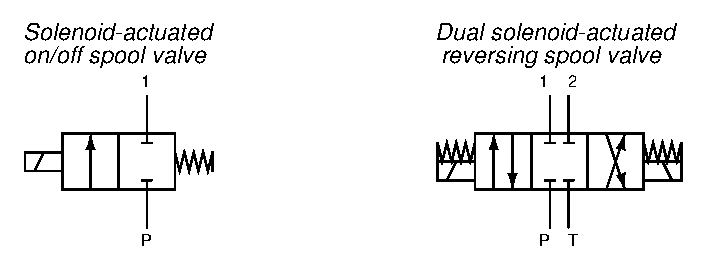
\includegraphics[width=15.5cm]{i00753x01.eps}$$

Forklar hva disse symbolene representerer, og hvordan de skal tolkes. Kommenter også hvordan en spoolventil er bygget opp.

\underbar{file i00753}
%(END_QUESTION)





%(BEGIN_ANSWER)

Symbolene viser hver ventils «normalstilling» (ikke aktivert). For å forstå hva som skjer når ventilen aktiveres, må du se for deg at boksene glir sidelengs slik at de kommer i linje med inn-/utløpsrørene, slik:

$$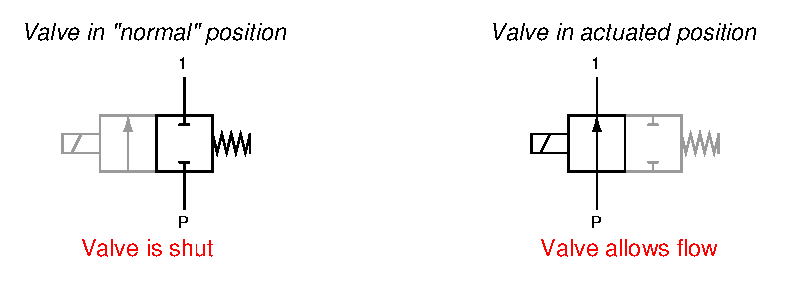
\includegraphics[width=15.5cm]{i00753x02.eps}$$

Det samme gjelder reverseringsventilen, bortsett fra at den har tre posisjoner:

$$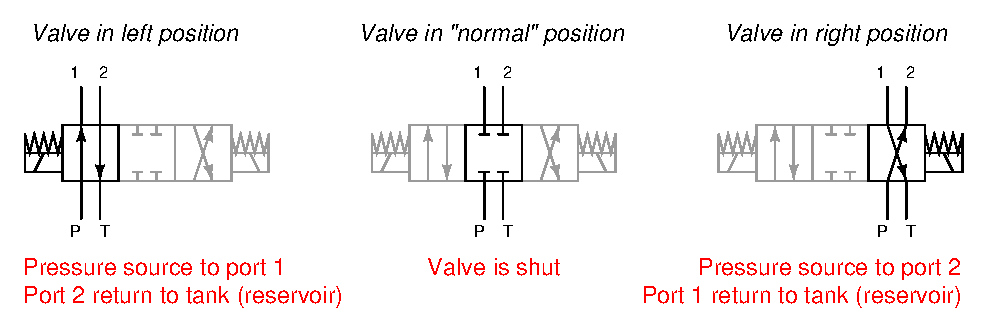
\includegraphics[width=15.5cm]{i00753x03.eps}$$

%(END_ANSWER)





%(BEGIN_NOTES)

Retningsventiler i hydraulikksystemer bruker ofte disse portbetegnelsene:

\begin{itemize}
\item{} P = Trykkilde (fra pumpe)
\item{} T = Retur til tank (reservoar)
\item{} 1 = Til den ene siden av sylinderen
\item{} 2 = Til den andre siden av sylinderen
\end{itemize}

Noen ganger brukes bokstavene «A» og «B» i stedet for tallene «1» og «2» for å betegne forbindelsene til hydraulikksylinderen.

%INDEX% Mekanikk, fluidkraftsystemer: symboler for spoolventiler

%(END_NOTES)


